\documentclass[twocolumn]{IEEEtran}
\usepackage[utf8]{inputenc}
\usepackage{graphicx}
\graphicspath{{figs/}} % No modificar
\usepackage{float}
\usepackage[spanish, es-tabla]{babel} % Configura el idioma a español
\addto\captionsspanish{\renewcommand{\figurename}{Figura}}
\addto\captionsspanish{\renewcommand{\tablename}{Tabla}}
\usepackage{subcaption}
\usepackage{hyperref}
\hypersetup{
    colorlinks=true,
    linkcolor=blue, % Cambia el color del número si lo deseas
    urlcolor=blue,
}

% \usepackage{ulem}
% http://ctan.org/pkg/{algorithms,algorithmx}
% \usepackage{algorithms,algorithmx}
\renewcommand{\thetable}{\arabic{table}}

\usepackage{hyperref}
\hypersetup{
    colorlinks=true,
    linkcolor=blue,
    filecolor=magenta,      
    urlcolor=blue,
    citecolor = blue,
}
\usepackage{tikz}

\newcommand{\hilight}[1]{\colorbox{yellow}{#1}}
%\numberwithin{equation}{section}
\usepackage{booktabs}
\usepackage{xcolor}
\usepackage{multirow}
\newtheorem{theorem}{Theorem}[section]
\makeatletter
\newcommand{\settheoremtag}[1]{% \settheoremtag{<tag>}
  \let\oldthetheorem\thetheorem% Store \thetheorem
  \renewcommand{\thetheorem}{#1}% Redefine it to a fixed value
  \g@addto@macro\endtheorem{% At \end{theorem}, ...
    \addtocounter{theorem}{-1}% ...restore theorem counter value and...
    \global\let\thetheorem\oldthetheorem}% ...restore \thetheorem
  }
\usepackage{titlesec}

% Cambiar tamaño de las secciones
\titleformat{\section}
  {\normalsize\bfseries}   % tamaño y estilo (large = un poco más grande que normal)
  {\thesection}{1em}  % numeración
  {}

\titleformat{\subsection}
  {\normalsize\bfseries} % tamaño de subsección
  {\thesubsection}{1em}
  {}

% PASO 1. Reemplace "Práctica 1" por el número de la práctica que corresponda
\newcommand{\dochead}{Laboratorio 3}     

% PASO 2. Verifique el título de la práctica corresponda.
\newcommand{\docsubhead}{PSD de señales aleatorias (GNU Radio)}  

% PASO 3. Reemplace "B1A - 02" por el grupo de la asignatura y el número de su grupo de laboratorio
\newcommand{\teamname}{A1L}     

% PASO 4. OPCIONAL: Reemplace "\docsubhead \docsubhead" por el título del documento en caso de requerirse.
\newcommand{\titulo}{\dochead: \docsubhead}      

% PASO 5. Reemplace "31 de diciembre de 2030" por la fecha de su documento
\newcommand{\fecha}{Septiembre 13, 2026}     

\input{./plantilla.tex}             % No modificar
\renewcommand{\lstlistingname}{Listado}

\usepackage{titlesec}
\titlespacing*{\section}
{0pt}{1ex}{1ex}  % Ajusta el espacio antes y después de las secciones

\usepackage[hidelinks]{hyperref}
\begin{document}  

% No modificar

\title{\vspace{1cm}\textbf{\titulo}}            % No modificar

% PASO 6. Agregar aquí el nombre y código de los autores.  
\author{
Andrés Felipe Flórez Quiroga - 2230399 \\
Edgar Joel Lizarazo Perez - 2234046
}
\affil{\small{\url{https://github.com/Andr3s-F/2026_2_CommII_A1L}}}
\affil{\normalsize{Escuela de Ingenierías Eléctrica, Electrónica y de Telecomunicaciones} \\ % No modificar
\small{Universidad Industrial de Santander}} % No modificar

\date{\today}

\maketitle                          % No modificar
\thispagestyle{fancy}               % No modificar

%---------------------------------------------------------------

\renewcommand{\abstractname}{Abstract}
\begin{abstract}
This report measures the power spectral density of random binary signals in GNU Radio. The number of samples per symbol was swept over 1, 4, 8 and 16 on a rectangular bipolar NRZ source, and the averaged periodogram was compared against a discrete time model based on the Dirichlet kernel instead of the usual continuous squared sinc. The peak held at 31.25 uW/Hz in the four runs, matching the predicted 1/Rb, and the spectral nulls stayed at multiples of 32 kHz. The first side lobe, on the other hand, dropped from 2.29 to 1.45 uW/Hz as Sps grew, a dependence the continuous model does not describe. Additive white Gaussian noise measured close to 3.9 uW/Hz against 3.906 uW/Hz expected. Bits taken from a JPEG file reproduced the ideal envelope, while an 8 bit PCM audio file added a comb of discrete lines spaced 4.12 kHz, consistent with the one byte period of each audio sample.
\end{abstract}

\begin{IEEEkeywords}
Densidad espectral de potencia, señales binarias aleatorias, núcleo de Dirichlet, periodograma promediado, ruido blanco gaussiano, codificación NRZ.
\end{IEEEkeywords}

\section{Introducción}

La densidad espectral de potencia describe cómo se reparte la potencia de una señal a lo largo de la frecuencia, y en comunicaciones digitales sirve para saber cuánto ancho de banda ocupa una transmisión antes de montarla. Para una señal binaria bipolar de forma rectangular el resultado clásico es un sinc al cuadrado con nulos en los múltiplos de la rata de bits \cite{b1}.

Ese resultado vale para pulsos continuos. GNU Radio trabaja con muestras, y el pulso rectangular se construye con un filtro interpolador cuyos coeficientes son unos, de modo que lo que aparece en pantalla no es exactamente un sinc al cuadrado. La diferencia se nota en los lóbulos laterales y depende de cuántas muestras por símbolo se usen. Medirla fue lo más interesante de esta práctica.

El montaje entregado con la guía \cite{b4} incluye una cadena de instrumentación que calcula la PSD por periodograma promediado. Sobre ese archivo se hizo el barrido de muestras por símbolo, se observó el ruido blanco gaussiano y se reemplazó la fuente aleatoria por dos archivos reales, una fotografía y una grabación de audio.

\section{Metodología}

\subsection{Montaje base y puntos de medida}

La fuente entrega bytes con valor 0 o 1 a una rata $R_b = 32$ kbit/s. Un bloque \textit{Char to Float} los convierte a punto flotante y define el punto de medida p3. La conversión a bipolar la hacen dos bloques en cascada, una suma con la constante $-0.5$ y una multiplicación por 2, que juntas implementan

\begin{equation}
    m[n] = 2\left(x[n] - \tfrac{1}{2}\right), \qquad x[n] \in \{0,1\}.
    \label{eq:bipolar}
\end{equation}

El \textit{Interpolating FIR Filter} recibe esa secuencia con interpolación igual a $Sps$ y coeficientes $h$, un vector de unos de longitud $Sps$. Inserta $Sps-1$ ceros entre símbolos y les aplica $h$, así que cada bit queda representado por $Sps$ muestras iguales de amplitud unitaria. A la salida la rata de muestreo es $f_s = R_b \cdot Sps$ y el punto se etiqueta como p4. Cambiar la interpolación sin cambiar $h$ rompe esa relación y la forma rectangular se pierde.

Una fuente de ruido gaussiano de amplitud unitaria alimenta un tercer punto, p5, que en el archivo original queda desconectado de los instrumentos.

La instrumentación agrupa las $N = 1024$ muestras en vectores, les aplica una FFT con ventana rectangular, toma la magnitud al cuadrado, promedia los vectores sucesivos y escala el resultado por $1/(N f_s)$. Eso es un periodograma promediado,

\begin{equation}
    \hat{S}(f_k) = \frac{1}{N f_s}\,\overline{|X_k|^2},
    \label{eq:periodograma}
\end{equation}

y entrega la PSD directamente en watts por hercio. La resolución del analizador queda fijada por

\begin{equation}
    \Delta f = \frac{f_s}{N}.
    \label{eq:resolucion}
\end{equation}

\subsection{Modificaciones al flujograma entregado}

El trabajo se hizo sobre tres versiones del archivo base, cada una con un cambio distinto. Las dos primeras aparecen en la Figura \ref{fig:diagramas}.

Para observar el ruido se intercambiaron las etiquetas de los dos bloques \textit{Virtual Source} de la zona de instrumentos, de manera que la cadena de medición lee p5 y la señal binaria se descarta en el \textit{Null Sink}, como muestra la Figura \ref{fig:diag_ruido}. La rama de ruido no pasa por ningún \textit{Throttle}, a diferencia de la rama de señal, de modo que corre a la velocidad que aguante el procesador. La lectura de la PSD no se altera por eso, ya que la normalización de la ecuación \eqref{eq:periodograma} usa el valor declarado de $f_s$ y no la rata real de ejecución.

Para los puntos de fuente real se deshabilitó el \textit{Random Source} en lugar de borrarlo, con lo que el archivo conserva el estado original a la vista, y en su lugar se conectó un \textit{File Source} de tipo byte seguido de un \textit{Unpack K Bits} con $K = 8$, según la Figura \ref{fig:diag_imagen}. El primero lee el archivo crudo y el segundo separa cada byte en ocho muestras de un bit, que es lo que espera el \textit{Char to Float}. La rata a la salida del desempaquetador es ocho veces la de entrada.

\begin{figure*}[!t]
    \centering
    \begin{subfigure}{0.46\textwidth}
        \centering
        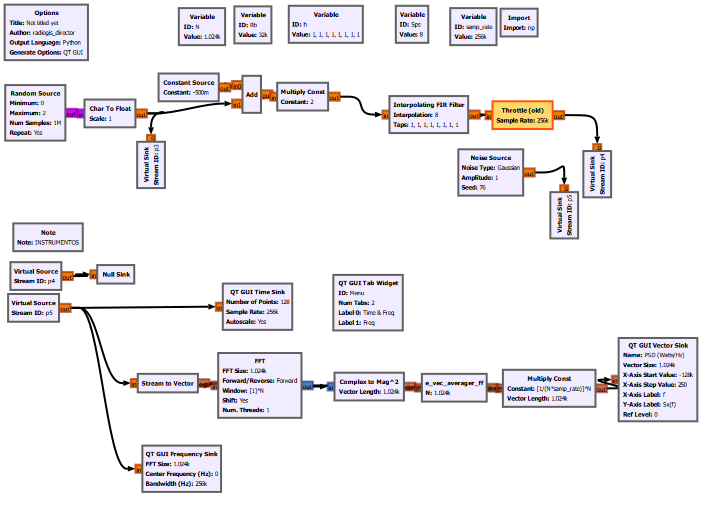
\includegraphics[width=\linewidth]{punto3_ruido.png}
        \caption{Instrumentación conmutada a p5 para observar el ruido.}
        \label{fig:diag_ruido}
    \end{subfigure}
    \hfill
    \begin{subfigure}{0.46\textwidth}
        \centering
        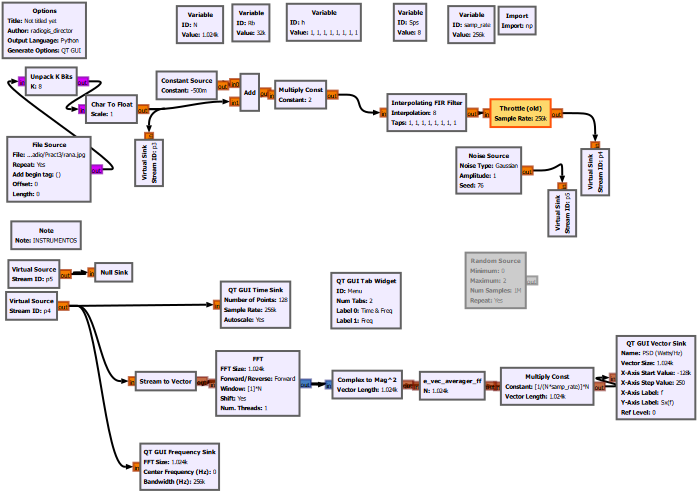
\includegraphics[width=\linewidth]{punto4_imagen.png}
        \caption{Fuente de archivo y desempaquetado de bits.}
        \label{fig:diag_imagen}
    \end{subfigure}
    \caption{Modificaciones aplicadas al flujograma de la guía \cite{b4}.}
    \label{fig:diagramas}
\end{figure*}

\subsection{Modelo teórico de la PSD}

Para símbolos $\pm 1$ independientes conformados por un pulso rectangular discreto de $Sps$ muestras, la respuesta del conformador es un núcleo de Dirichlet \cite{b3} y la densidad espectral bilateral queda

\begin{equation}
    S(f) = \frac{1}{R_b\,Sps^2}\left|\frac{\sin(\pi f / R_b)}{\sin(\pi f / f_s)}\right|^{2}.
    \label{eq:psd}
\end{equation}

De la ecuación \eqref{eq:psd} salen tres predicciones que permiten verificar cada corrida. El valor en el origen vale $1/R_b$ sin importar $Sps$, porque el numerador y el denominador crecen juntos. Los nulos caen donde se anula el numerador, en $f = k R_b$ con $k$ entero. Y como la pantalla abarca de $-f_s/2$ a $f_s/2$, el número de lóbulos visibles resulta

\begin{equation}
    N_{lob} = \frac{f_s}{R_b} = Sps,
    \label{eq:lobulos}
\end{equation}

contando el central como dos por tener el doble de ancho. El caso $Sps = 1$ es especial: los dos senos se cancelan y la PSD queda constante en $1/R_b$.

Para el ruido gaussiano de desviación $\sigma$ la densidad esperada es plana con valor $\sigma^2/f_s$.

\subsection{Revisión del algoritmo del promediador}

El bloque de Python que promedia los vectores viene con la guía y usa la interfaz de bloque embebido de GNU Radio \cite{b2}. Una revisión línea por línea antes de usarlo dejó ver los defectos de la Tabla \ref{tab:correcciones}. Ninguno impide la ejecución, pero los dos primeros sesgan la lectura durante el transitorio y el tercero obliga a reiniciar el diagrama cada vez que cambia un parámetro.

\begin{table}[!ht]
\centering
\caption{Defectos del algoritmo entregado y corrección propuesta.}
\label{tab:correcciones}
\scriptsize
\begin{tabular}{@{}p{1.3cm}p{2.8cm}p{2.8cm}@{}}
\toprule
\textbf{Aspecto} & \textbf{Código base} & \textbf{Corrección} \\
\midrule
Promedio por fila & Todas las filas del bloque reciben el mismo promedio final, ya dividido por el contador incrementado & \texttt{np.cumsum} sobre las filas, cada vector con su propio divisor \\
Estado inicial & \texttt{self.sum} arranca como escalar entero y se convierte en vector por difusión & \texttt{np.zeros(N)} en \texttt{float64} desde el constructor \\
Memoria & Acumula desde el arranque y nunca olvida & Factor de olvido exponencial \texttt{alpha} opcional \\
\bottomrule
\end{tabular}
\end{table}

La versión corregida aparece en el Listado \ref{lst:promediador}. Con \texttt{alpha} en cero reproduce el promedio acumulado del original, ya sin el sesgo por fila, y con valores pequeños se comporta como una ventana exponencial de longitud efectiva $1/\alpha$.

\lstset{language=Python, basicstyle=\scriptsize\ttfamily}
\begin{lstlisting}[caption={Promediador de vectores con corrección por fila y olvido opcional.},label={lst:promediador},numbers=none,xleftmargin=6pt,framexleftmargin=4pt,breaklines=false]
def work(self, input_items, output_items):
    x, y = input_items[0], output_items[0]
    a = self.alpha
    if a > 0.0:
        for i in range(len(x)):
            self.acum = (1-a)*self.acum + a*x[i]
            y[i] = self.acum
    else:
        s = np.cumsum(x, axis=0,
                      dtype=np.float64)
        s += self.acum
        n = self.filas + np.arange(1, len(x)+1)
        y[:] = s / n[:, None]
        self.acum = s[-1]
    self.filas += len(x)
    return len(y)
\end{lstlisting}

Las medidas de este informe se tomaron con el algoritmo original. Para evitar el sesgo sin modificar el bloque se esperó la convergencia de la traza antes de capturar y se reinició el diagrama entre configuraciones, ya que el acumulador conserva el historial del valor anterior.

\section{RESULTADOS Y ANÁLISIS DE DATOS}

\subsection{Barrido de muestras por símbolo}

El montaje se corrió con $h$ de longitud 1, 4, 8 y 16, dejando $R_b$ fijo. La Figura \ref{fig:barrido} reúne las cuatro salidas y la Tabla \ref{tab:barrido} compara las lecturas contra el modelo.

\begin{figure*}[!t]
    \centering
    \begin{subfigure}{0.46\textwidth}
        \centering
        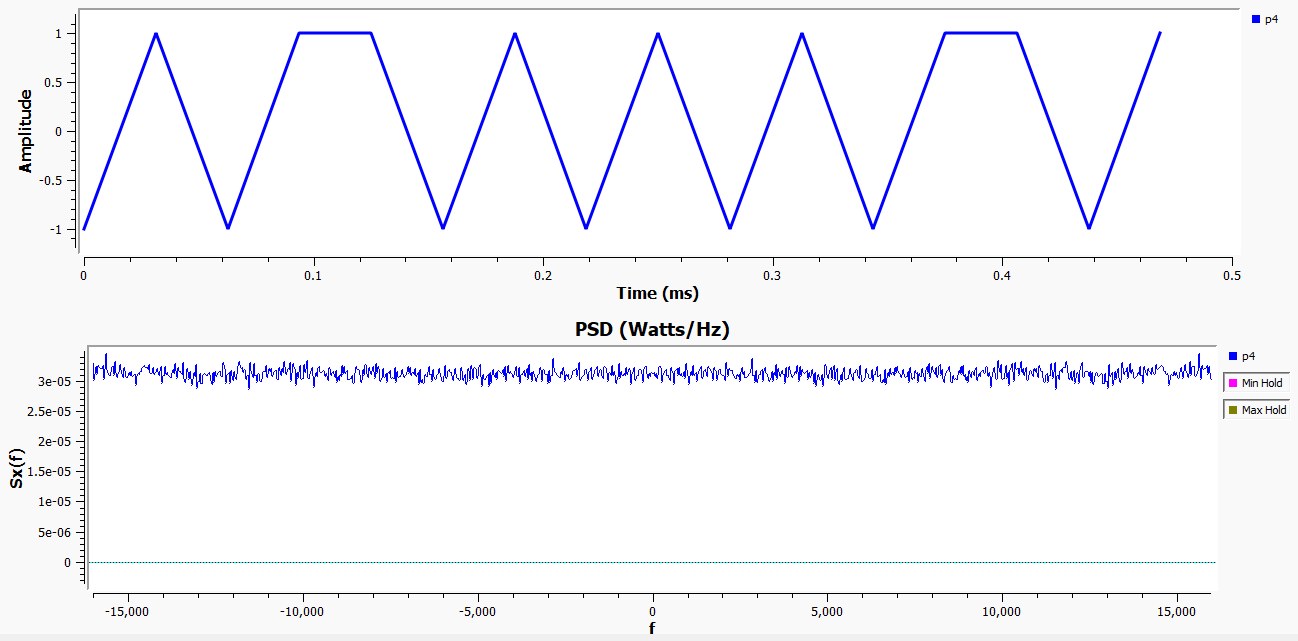
\includegraphics[width=\linewidth]{sps_1_amp_psd.png}
        \caption{$Sps = 1$}
        \label{fig:sps1}
    \end{subfigure}
    \hfill
    \begin{subfigure}{0.46\textwidth}
        \centering
        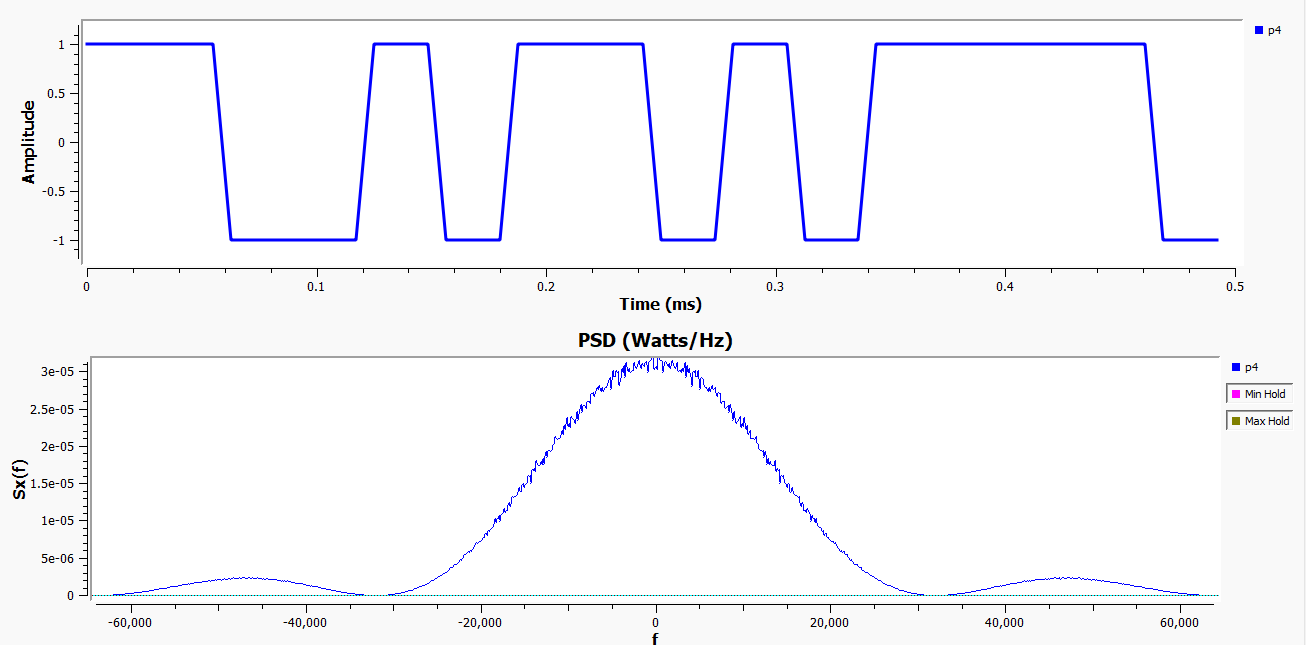
\includegraphics[width=\linewidth]{sps_4_amp_psd.png}
        \caption{$Sps = 4$}
        \label{fig:sps4}
    \end{subfigure}
    \\[0.15cm]
    \begin{subfigure}{0.46\textwidth}
        \centering
        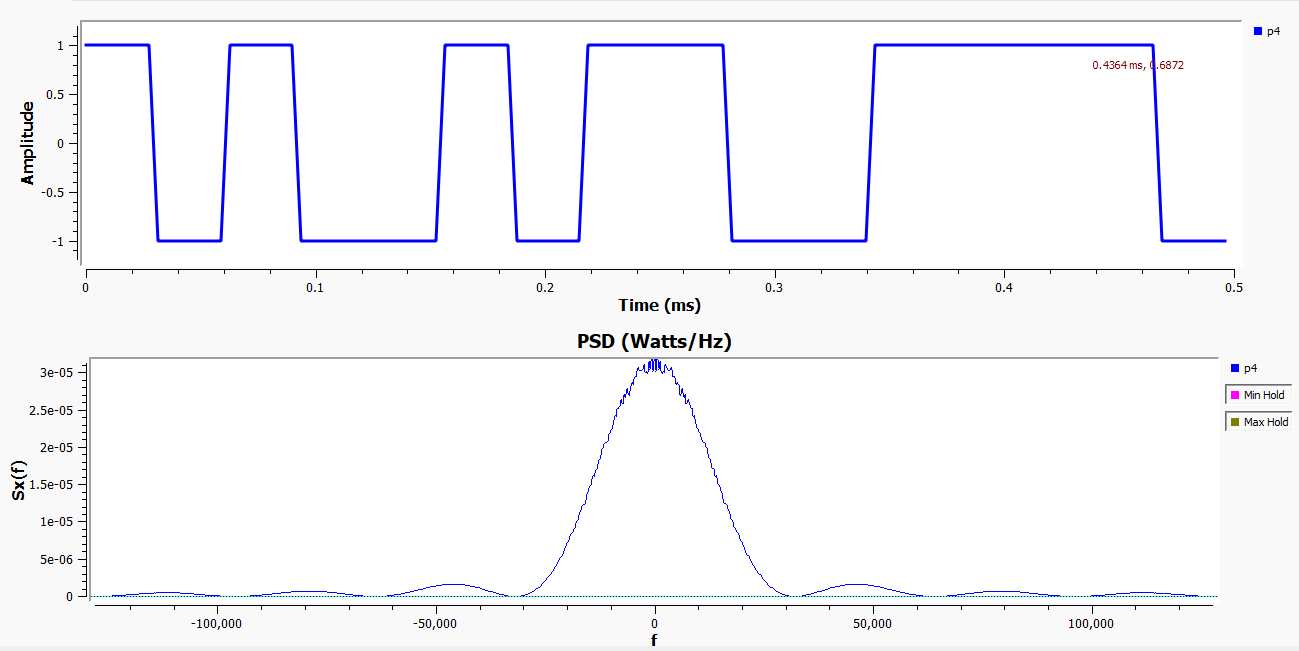
\includegraphics[width=\linewidth]{sps_8_amp_psd.png}
        \caption{$Sps = 8$}
        \label{fig:sps8}
    \end{subfigure}
    \hfill
    \begin{subfigure}{0.46\textwidth}
        \centering
        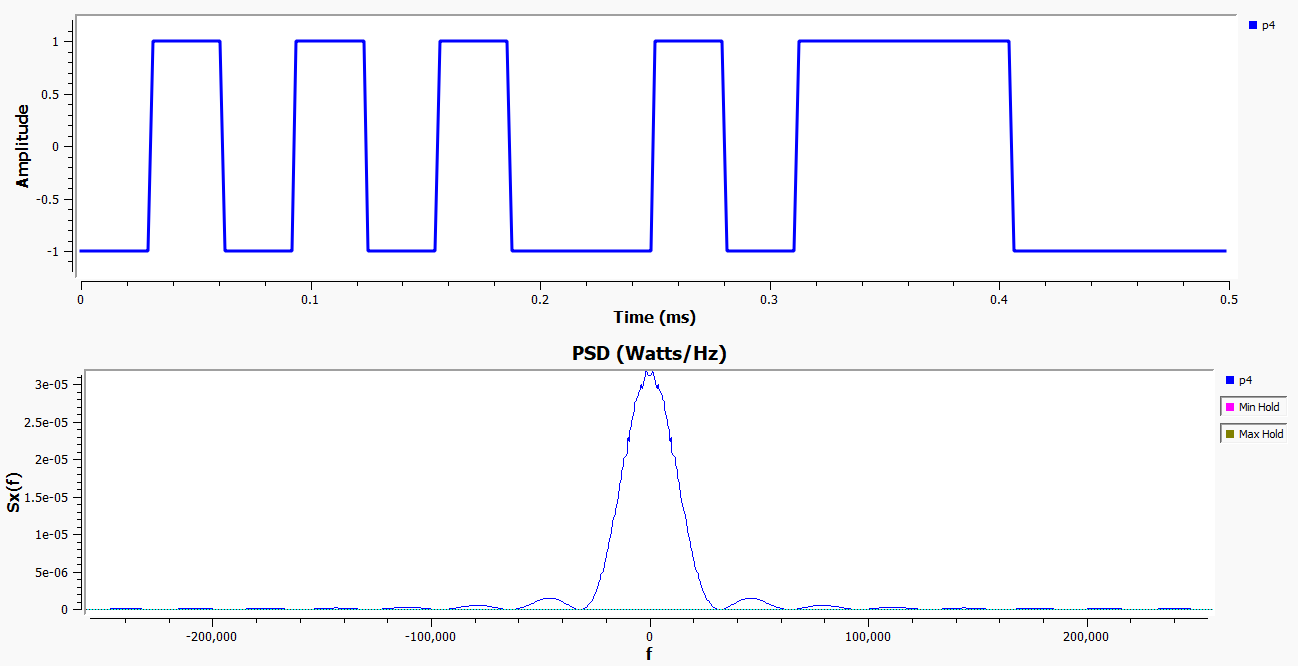
\includegraphics[width=\linewidth]{sps_16_amp_psd.png}
        \caption{$Sps = 16$}
        \label{fig:sps16}
    \end{subfigure}
    \caption{Señal en el tiempo y PSD de la señal binaria bipolar para las cuatro configuraciones del conformador.}
    \label{fig:barrido}
\end{figure*}

\begin{table}[!ht]
\centering
\caption{Parámetros del barrido, con $R_b = 32$ kbit/s en las cuatro corridas. El pico y el lóbulo lateral están en $\mu$W/Hz.}
\label{tab:barrido}
\footnotesize
\begin{tabular}{@{}lrrrrrr@{}}
\toprule
 & $f_s$ & $\Delta f$ & $BW$ & \multicolumn{2}{c}{\textbf{Pico}} & \textbf{Lób.} \\
\cmidrule(lr){5-6}
$Sps$ & (kHz) & (Hz) & (kHz) & Teór. & Med. & Teór. \\
\midrule
1  & 32  & 31.25 & 16 & 31.25 & 31 & plano \\
4  & 128 & 125   & 32 & 31.25 & 31 & 2.29 \\
8  & 256 & 250   & 32 & 31.25 & 31 & 1.58 \\
16 & 512 & 500   & 32 & 31.25 & 31 & 1.45 \\
\bottomrule
\end{tabular}
\end{table}

El pico se mantuvo pegado al borde superior de la escala en las cuatro corridas. Ese borde está fijado en $1/R_b = 31.25\ \mu$W/Hz por configuración del \textit{Vector Sink}, así que la coincidencia con la ecuación \eqref{eq:psd} se lee de forma directa sobre la gráfica. Multiplicar por cuatro el número de muestras por símbolo no cambió la altura del lóbulo principal.

Los nulos tampoco se movieron. En las Figuras \ref{fig:sps4}, \ref{fig:sps8} y \ref{fig:sps16} el primero cae en $\pm 32$ kHz, que es $R_b$, aunque el eje de frecuencia se extienda al doble en cada paso. Lo que cambia es cuántos alcanzan a verse dentro de la ventana. El conteo dio 4, 8 y 16 lóbulos respectivamente, tal como predice la ecuación \eqref{eq:lobulos}. El ancho de banda de primer nulo vale entonces $R_b = 32$ kHz en esas tres configuraciones, sin importar la frecuencia de muestreo. Con $Sps = 1$ no hay ningún nulo dentro de la pantalla y la señal ocupa toda la banda disponible, es decir $f_s/2 = 16$ kHz, que es el valor reportado en la Tabla \ref{tab:barrido}.

Con $Sps = 1$ la señal deja de tener forma rectangular. Cada bit ocupa una sola muestra y el \textit{Time Sink} une los puntos con rectas, de ahí el zigzag triangular de la Figura \ref{fig:sps1} con mesetas donde se repiten dos bits iguales. La PSD sale plana en todo el intervalo, con un rizado de alrededor del diez por ciento que corresponde a la varianza del periodograma. Una secuencia de muestras $\pm 1$ independientes es ruido blanco en tiempo discreto, y por eso su espectro no se distingue en forma del que produce la fuente gaussiana.

Los lóbulos laterales sí dependen de $Sps$, y ese comportamiento no se anticipa desde el modelo continuo. Evaluando la ecuación \eqref{eq:psd} en $f = 1.5 R_b$, donde cae el primer lóbulo secundario, el modelo discreto da 2.29, 1.58 y 1.45 $\mu$W/Hz para $Sps$ de 4, 8 y 16. El sinc al cuadrado continuo predice 1.41 $\mu$W/Hz para los tres. La tendencia se observa en la Figura \ref{fig:barrido}: los lóbulos laterales de \ref{fig:sps4} son claramente más altos que los de \ref{fig:sps16}, con \ref{fig:sps8} en medio. El motivo es geométrico. Con pocas muestras por símbolo el pulso discreto se aparta del rectángulo ideal, y el denominador $\sin(\pi f / f_s)$ de la ecuación \eqref{eq:psd} todavía no puede aproximarse por su argumento. A medida que $Sps$ crece esa aproximación mejora y el resultado tiende al caso continuo.

\subsection{Ruido blanco gaussiano}

Con la instrumentación conmutada a p5 y $Sps = 8$ se obtuvo la Figura \ref{fig:ruido}. La traza temporal no tiene niveles discretos y alcanza excursiones de $\pm 3$, coherentes con una distribución gaussiana de desviación unitaria.

\begin{figure}[!ht]
    \centering
    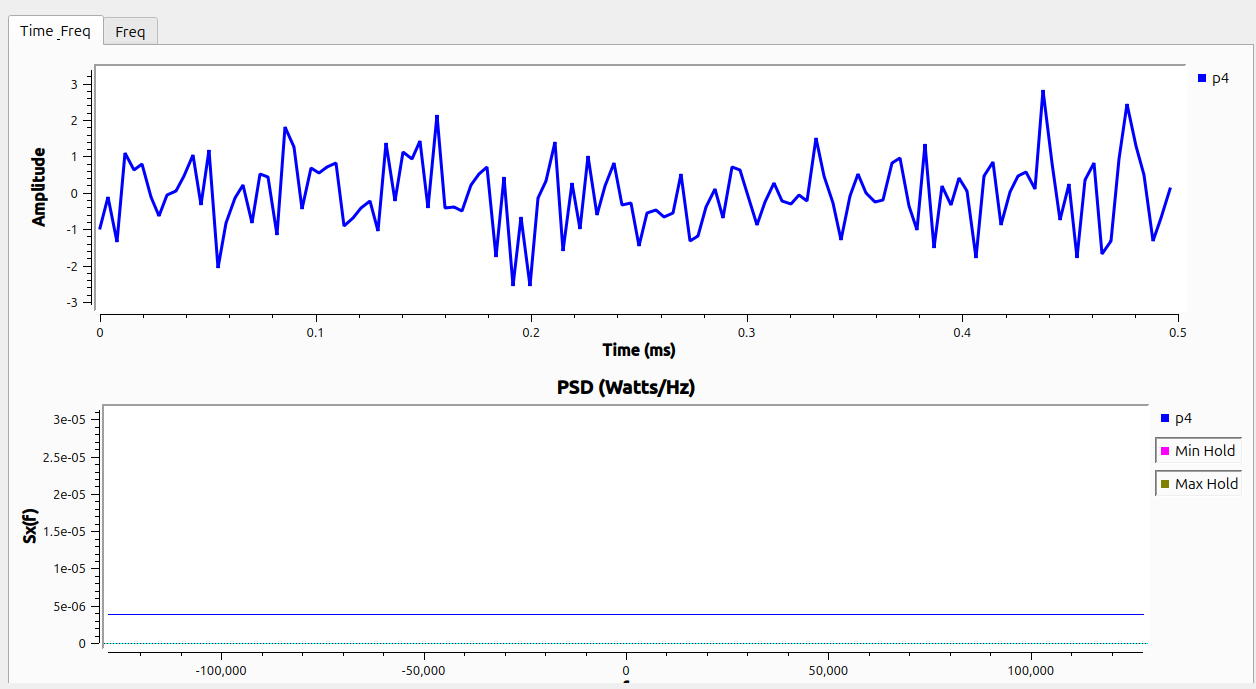
\includegraphics[width=\linewidth]{ruido_tiempo_psd.png}
    \caption{Ruido blanco gaussiano en tiempo y su PSD, medido con $Sps = 8$.}
    \label{fig:ruido}
\end{figure}

La PSD medida quedó ligeramente por debajo de la marca de 5 $\mu$W/Hz, contra los $\sigma^2/f_s = 3.906\ \mu$W/Hz esperados. Que la traza sea plana en toda la pantalla no contradice el ancho de banda infinito del ruido blanco teórico. El muestreo a $f_s$ pliega todo el contenido por encima de Nyquist hacia el intervalo visible, y la superposición de infinitas réplicas de un espectro plano sigue siendo plana.

Comparar esta figura con la Figura \ref{fig:sps1} deja ver un detalle útil. Las dos densidades son planas, pero la del ruido está ocho veces más abajo. Las dos señales tienen potencia total de 1 W, y esa potencia se reparte sobre $f_s$: 32 kHz en un caso y 256 kHz en el otro. La altura del piso espectral no dice nada por sí sola si no se conoce la rata de muestreo.

\subsection{Bits provenientes de fuentes reales}

La fuente aleatoria se reemplazó por los dos archivos de la guía y el resto del montaje quedó igual. Los resultados están en la Figura \ref{fig:fuentes}.

\begin{figure*}[!t]
    \centering
    \begin{subfigure}{0.46\textwidth}
        \centering
        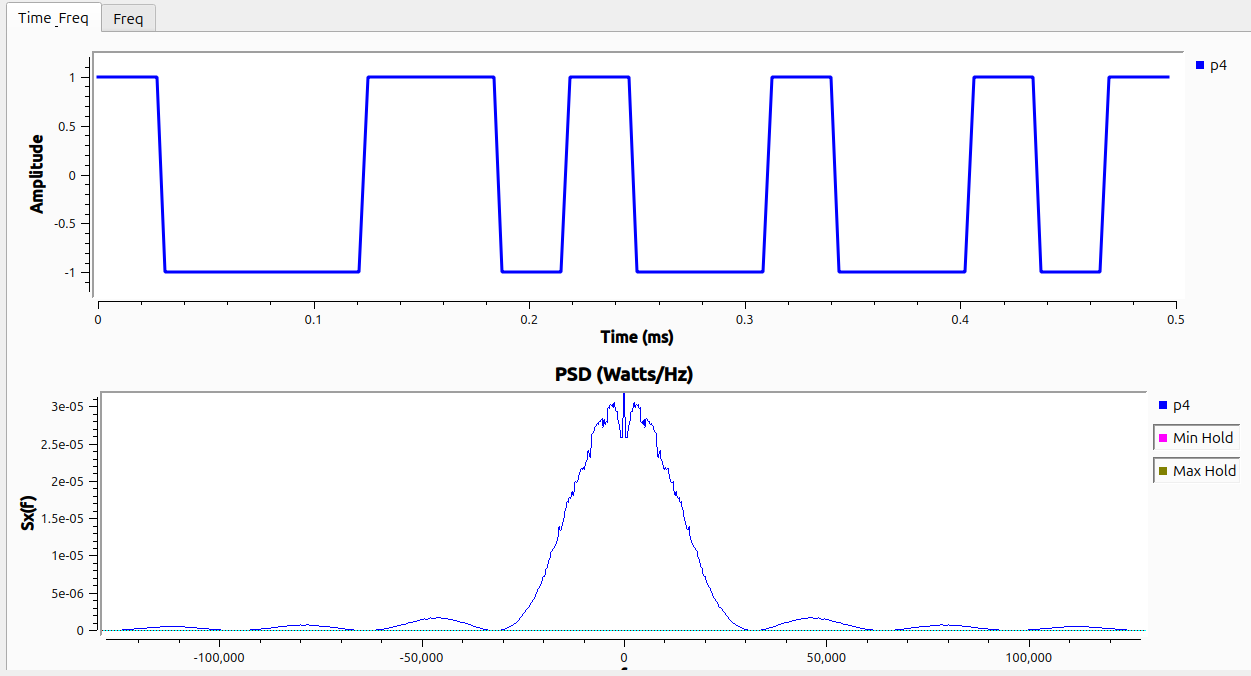
\includegraphics[width=\linewidth]{rana_tiempo_psd.png}
        \caption{Bits de la imagen \texttt{rana.jpg}.}
        \label{fig:rana}
    \end{subfigure}
    \hfill
    \begin{subfigure}{0.46\textwidth}
        \centering
        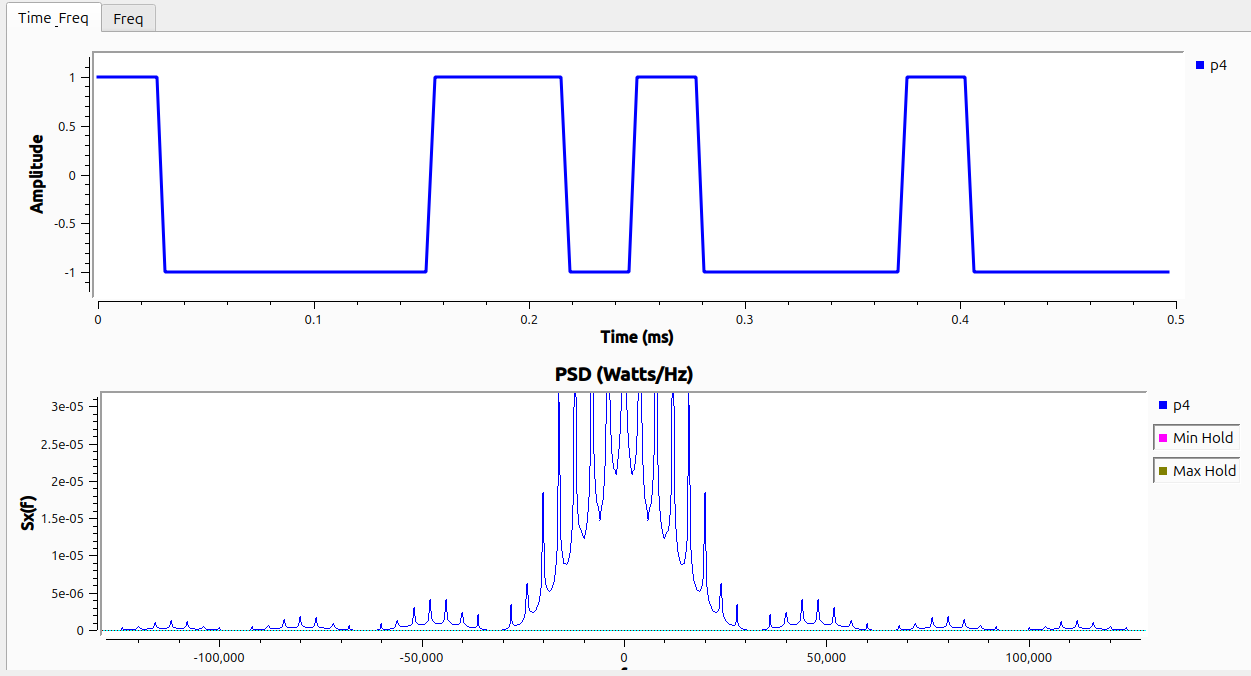
\includegraphics[width=\linewidth]{sonido_tiempo_psd.png}
        \caption{Bits del audio \texttt{sonido.wav}.}
        \label{fig:sonido}
    \end{subfigure}
    \caption{Señal en el tiempo y PSD cuando los bits provienen de archivos reales, con $Sps = 8$.}
    \label{fig:fuentes}
\end{figure*}

La imagen produjo un espectro casi idéntico al de la fuente aleatoria. En la Figura \ref{fig:rana} el lóbulo principal alcanza el mismo pico de 31 $\mu$W/Hz, los nulos siguen en $\pm 32$ kHz y los lóbulos laterales conservan la altura del caso $Sps = 8$. Un JPEG está comprimido, y la compresión funciona justamente eliminando la redundancia del archivo, así que sus bytes se acercan bastante a una secuencia de bits equiprobables e independientes. La traza temporal lo confirma con transiciones frecuentes y pocas rachas largas.

El audio produjo un resultado distinto. La Figura \ref{fig:sonido} muestra un peine de líneas espectrales discretas que se levantan por encima de la envolvente, concentradas en el lóbulo principal y repetidas con menor amplitud en los laterales. Dos líneas vecinas medidas con el cursor dieron $-28033$ Hz y $-23916$ Hz, es decir un espaciado de 4.12 kHz.

Ese número identifica el origen del peine. El archivo es PCM mono de 8 bits sin comprimir, de modo que cada muestra de audio ocupa exactamente un byte y el \textit{Unpack K Bits} con $K = 8$ entrega una muestra completa por cada ocho bits de la secuencia. Una estructura que se repite cada $L$ bits aparece en el espectro como líneas separadas $R_b / L$, y con $L = 8$ eso da 4 kHz. La diferencia con los 4.12 kHz leídos es menor que la resolución del analizador, que en esta corrida vale 250 Hz según la ecuación \eqref{eq:resolucion}. Dentro de cada byte el bit más significativo cambia despacio, porque sigue la envolvente de la onda sonora, mientras que los menos significativos cambian casi en cada muestra. Esa periodicidad de ocho bits es la que produce las líneas.

En el tiempo la diferencia también se nota. Las rachas de bits iguales del audio son más largas que las de la imagen, lo que desplaza potencia hacia las frecuencias bajas. Las dos señales son binarias bipolares rectangulares y comparten envolvente, pero la envolvente solo describe la forma del pulso. Lo que le pasa a la PSD dentro de esa envolvente depende de la estadística de la fuente.

\section{Conclusiones}

\begin{itemize}

\item El pico de la densidad espectral se mantuvo en 31 $\mu$W/Hz frente a los 31.25 $\mu$W/Hz de $1/R_b$ en las cuatro configuraciones del conformador, y los nulos permanecieron en múltiplos de 32 kHz. Cambiar las muestras por símbolo redistribuye el espectro sobre un eje más ancho sin alterar ni la altura del lóbulo principal ni el ancho de banda de primer nulo.

\item El número de lóbulos visibles coincidió con el valor de $Sps$ en las tres configuraciones donde hay nulos dentro de la pantalla. La relación $N_{lob} = f_s / R_b$ permite estimar la rata de bits contando lóbulos cuando solo se conoce la frecuencia de muestreo.

\item La altura del primer lóbulo lateral bajó de 2.29 a 1.45 $\mu$W/Hz entre $Sps = 4$ y $Sps = 16$, acercándose a los 1.41 $\mu$W/Hz del modelo continuo. El sinc al cuadrado de la teoría clásica subestima los lóbulos laterales cuando hay pocas muestras por símbolo, y el núcleo de Dirichlet describe esa desviación.

\item Con $Sps = 1$ la señal binaria bipolar tiene la misma densidad plana que el ruido blanco gaussiano, porque una secuencia de muestras independientes no tiene correlación entre muestras vecinas. Las dos densidades planas se diferencian en nivel por la razón entre sus frecuencias de muestreo, ocho veces en este caso.

\item Una fuente comprimida y una sin comprimir generan espectros distintos aunque compartan la misma forma de pulso. Los bits del JPEG reprodujeron la envolvente de la fuente aleatoria, mientras que los del WAV añadieron líneas discretas cada 4.12 kHz, valor que corresponde a $R_b/8$ y delata el byte de cada muestra PCM. La forma de la PSD combina el conformador de pulso con la estadística de la fuente, y para caracterizar un enlace no basta con conocer el primero.

\end{itemize}

% NO MODIFIQUE NI ELIMINE ESTA PARTE PARA QUE APAREZCAN LAS REFERENCIAS
\bibliographystyle{IEEEtran}

\begin{thebibliography}{00}

\bibitem{b1}
Escuela de Ingenierías Eléctrica, Electrónica y de Telecomunicaciones, 
\textit{Libro de Comunicaciones Plus Volumen I}. 
Bucaramanga, Colombia: Universidad Industrial de Santander, 2020, material de apoyo académico.

\bibitem{b2}
GNU Radio Project, ``Creating Your First Block,'' GNU Radio Wiki. [En línea]. Disponible: \url{https://wiki.gnuradio.org/index.php?title=Creating_Your_First_Block}

\bibitem{b3}
A. V. Oppenheim y R. W. Schafer, \textit{Discrete-Time Signal Processing}, 3a ed. Upper Saddle River, NJ, EE. UU.: Pearson, 2010.

\bibitem{b4}
O. J. Tíjaro Rojas, \textit{PSD de señales aleatorias (GNURadio)}, guía de laboratorio, Comunicaciones II (27145). Universidad Industrial de Santander, 2026.

\end{thebibliography}

\end{document}
